%!TEX root = ../../../main.tex

\section{Photoluminescence Spectra} \label{sec::spectra}

	To identify \nds containing \sivs, we performed confocal scans of the samples, see \Fref{fig::scans}. 
	To reduce bias in the measurements, not only the brightest spots of the confocal scans are investigated, but also those which barely exceed \bkg fluorescence.
	\sivs are further investigated by measuring \pl (PL) spectra, single photon statistics and photo-stability.
	As discussed in \Fref{ch::sivs}, the typical luminescence spectrum of an \siv is composed of a prominent \zpl peak and weak sidebands.
	Investigations of both are reported independently in the following paragraphs.

	\begin{figure}[!htb]
		\begin{subfigure}{ 0.49\linewidth}
			\centering
			\testbox{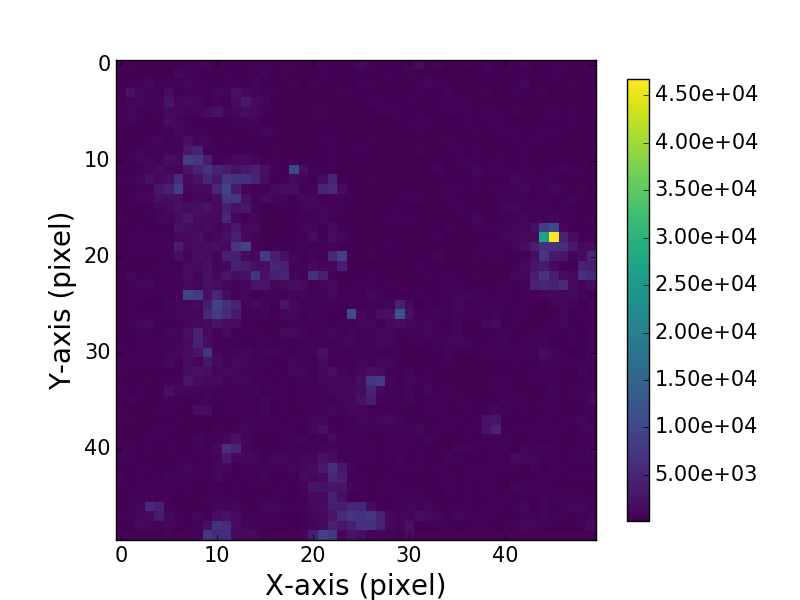
\includegraphics[trim = 0 0 0 0,  clip= true, width = \pairplotwide]{./pics/scan_xy-02_2APD.png}}
			\caption{}
			\label{subfig::scan_1}
		\end{subfigure}
		\hfill
		\begin{subfigure}{ 0.49\linewidth}
			\centering
			\testbox{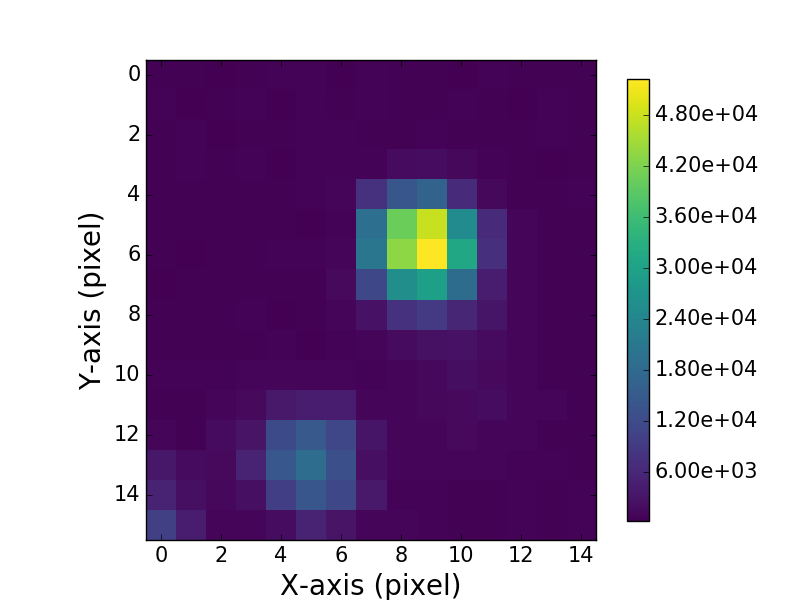
\includegraphics[trim = 0 0 0 0,  clip= true, width = \pairplotwide]{./pics/scan_xy-05_2APD.png}}
			\caption{}
			\label{subfig::scan_2}
		\end{subfigure}
		\caption[Confocal \pl scans]{\Pl scans measured in the confocal setup. (a) depicts an overview of a size of $\SI{50}{\micro\meter}\times\SI{50}{\micro\meter}$, The bright yellow dot is emitter \embroad introduced in this chapter. Also several of the not so intense emitter visible as light blue spots were investigated. (b) Shows a detail scan of a size of $\SI{8}{\micro\meter}\times\SI{7.5}{\micro\meter}$ of \embroad.}
		\label{fig::scans}
	\end{figure}

	\FloatBarrier	

\subsection{Zero-Phonon-Line}\label{subsec::zpl}

	The \cwl and the \lw of the \zpl (\ZPL) of \siv luminescence spectra for samples \insituF, \insituS, and \insituH are determined by fitting a Lorentzian fit to the \ZPL.
	Both spectra from \nds containing single and multiple \sivs are taken into account.
	\Fref{fig::various_spectra} depicts a few examples of the measured spectra in order show how diverse they are.

	\begin{figure}[!htb]
		\begin{subfigure}[t]{ 0.49\linewidth}
			\centering
			\testbox{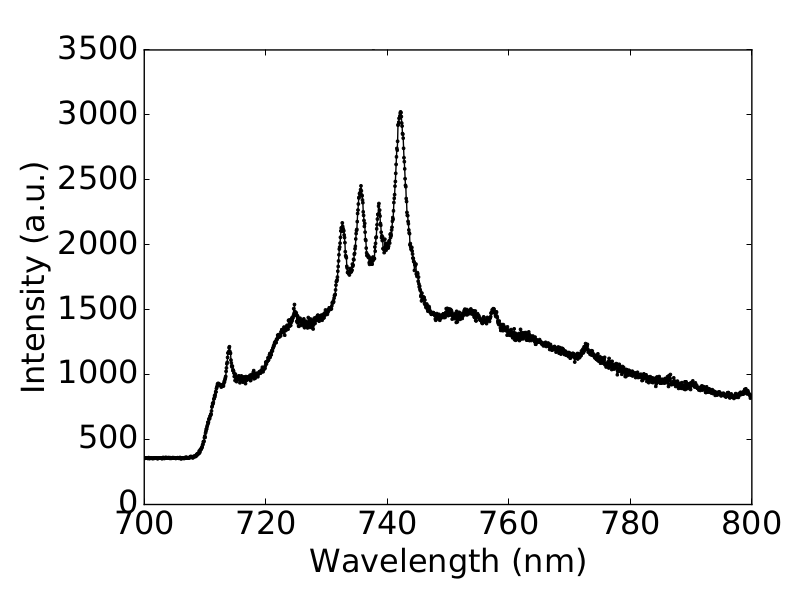
\includegraphics[trim = 0 0 0 0,  clip= true, width = \pairplotwide]{./pics/spectrum11.png}}
			\caption{}
			\label{subfig::spectrum_1}
		\end{subfigure}
		\hfill
		\begin{subfigure}[t]{ 0.49\linewidth}
			\centering
			\testbox{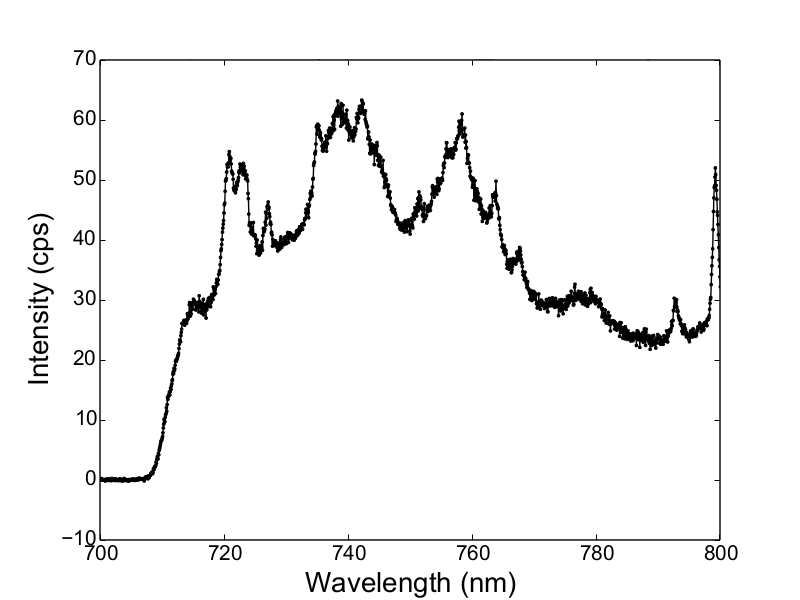
\includegraphics[trim = 0 0 0 0,  clip= true, width = \pairplotwide]{./pics/Spektrum3_t=30s.png}}
			\caption{}
			\label{subfig::spectrum_2}
		\end{subfigure}
		\hfill
		\begin{subfigure}[t]{ 0.49\linewidth}
			\centering
			\testbox{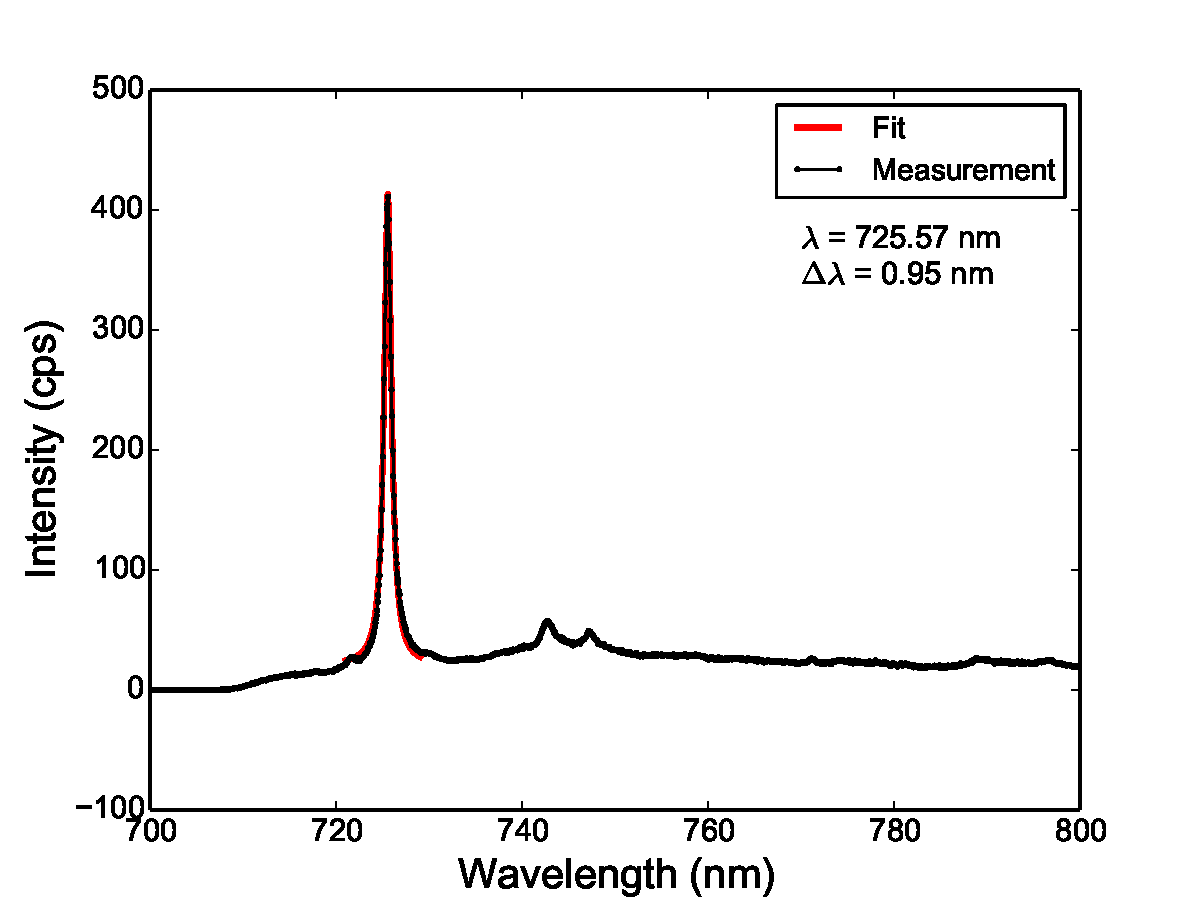
\includegraphics[trim = 0 0 0 0,  clip= true, width = \pairplotwide]{./pics/Spektrum2_2_t=30s_alt.pdf}}
			\caption{}
			\label{subfig::spectrum_3}
		\end{subfigure}
		\hfill
		\begin{subfigure}[t]{ 0.49\linewidth}
			\centering
			\testbox{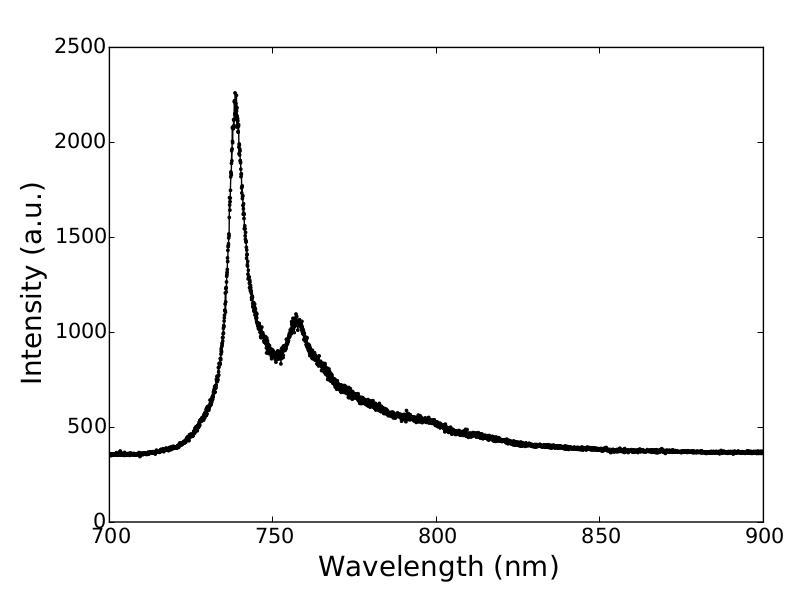
\includegraphics[trim = 0 0 0 0,  clip= true, width = \pairplotwide]{./pics/plot_spe_scan_xy-39x8y9_300uW_t120.png}}
			\caption{}
			\label{subfig::spectrum_4}
		\end{subfigure}
		\hfill
		\begin{subfigure}[t]{ 0.49\linewidth}
			\centering
			\testbox{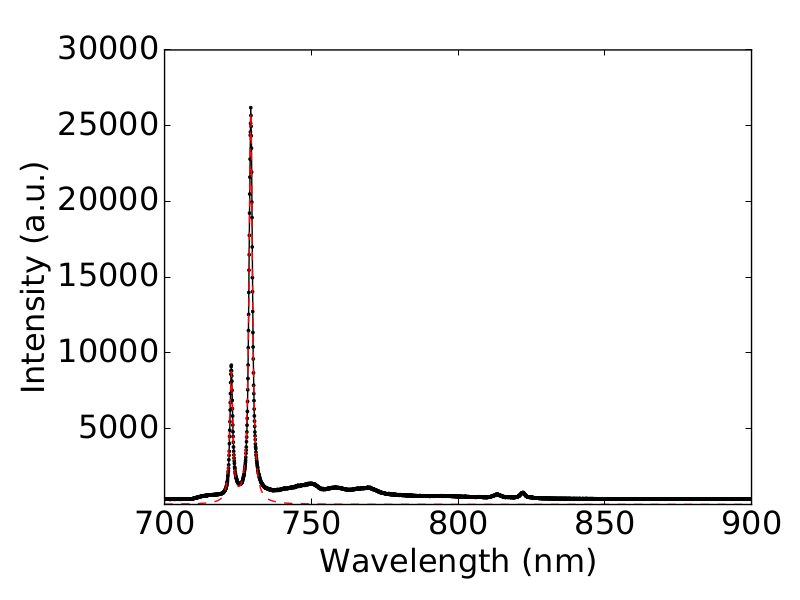
\includegraphics[trim = 0 0 0 0,  clip= true, width = \pairplotwide]{./pics/spectrum_scan_xy-40x4y4_392uW_t10_fit.png}}
			\caption{}
			\label{subfig::spectrum_5}
		\end{subfigure}
		\hfill
		\begin{subfigure}[t]{ 0.49\linewidth}
			\centering
			\testbox{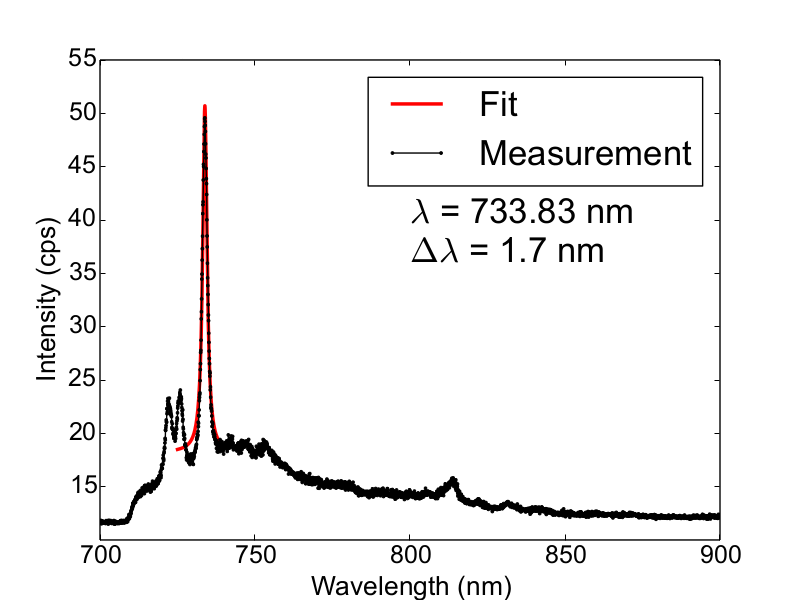
\includegraphics[trim = 0 0 0 0,  clip= true, width = \pairplotwide]{./pics/spectrum_scan_xy-21_2_t30_380uW.png}}
			\caption{}
			\label{subfig::spectrum_6}
		\end{subfigure}
		\caption[Overview of diversity of \siv spectra.]{Various spectra of samples consisting of wet-milled \nds with \textit{in-situ} incorporated \sivs. The \nds yielding spectra (a) and (b) host many \sivs with \ZPL at different \cwls. (c) and (d) exhibit one dominant \ZPL and recognizeable sideband features. In (e) two \ZPLs of different intensity are visible, in (f) one \ZPL donminates the spectrum while some \ZPLs of lower intensity are present.}
		\label{fig::various_spectra}
	\end{figure}

	In \Fref{fig::bimodal_distr} the \lw for each measured \ZPL is plotted against its \cwl.

	\begin{figure}[!htb]
			\centering
			\testbox{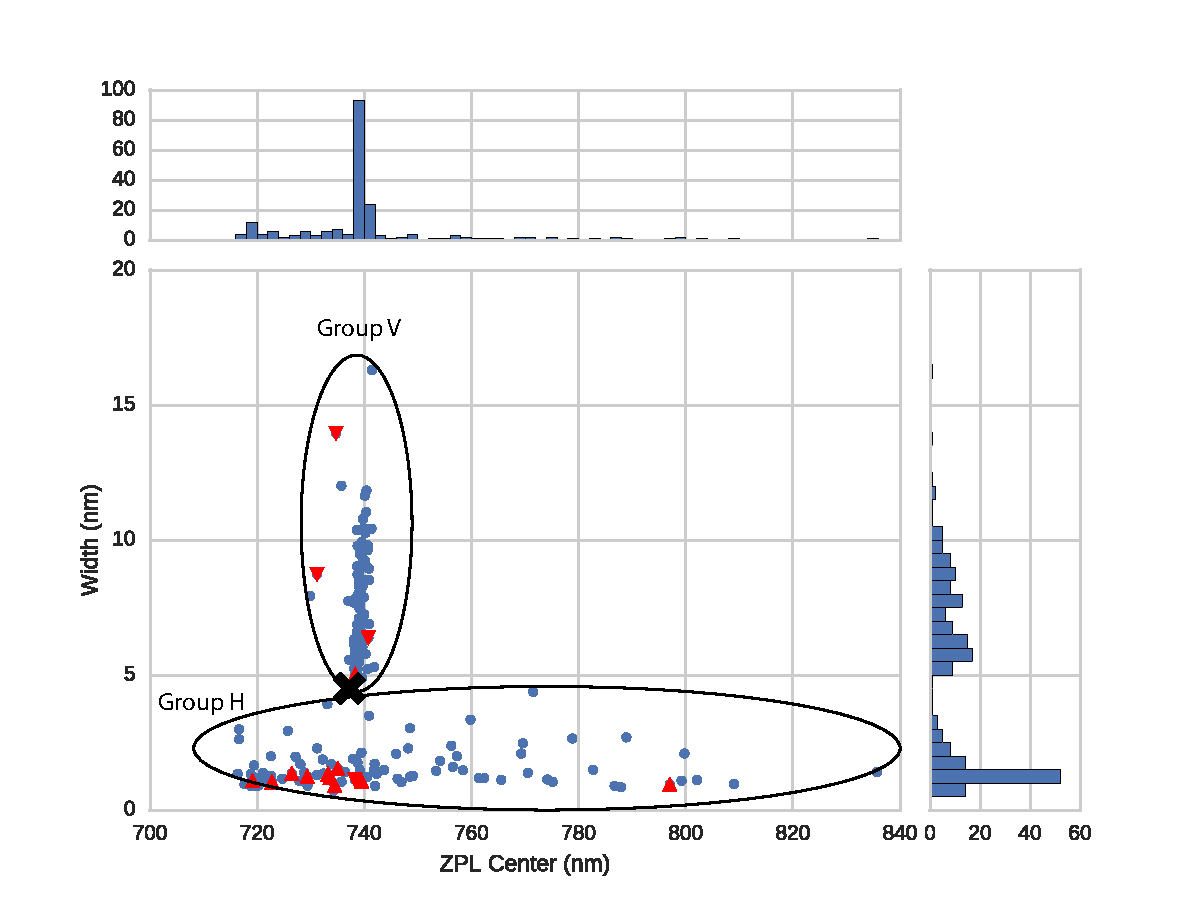
\includegraphics[trim = 0 0 0 0,  clip= true, width = \oneimagewide]{./pics/distro_histo_sarah.pdf}}
			\caption[Spectral distribution of \siv \ZPLs]{Distribution of the \ZPL \cwl versus the \lw of the \ZPL of the investigated \sivs in milled \nds containing \textit{in-situ} incorporated \sivs for samples \insituF, \insituS, \insituH{}. The data separates into a horizontal (\hl) and a vertical (\vl) cluster. The bold black cross marks the position of an ideal \siv in unstrained bulk diamond \cite{Arend2016a}. The red triangles indicate emitters with an anti-bunching dip in the \gtz measurement. Upwards pointing triangles represent blinking emitters (fluorescence intermittency), while triangles pointing down represent non-blinking emitters (see \Fref{subsec::photostab}).}
			\label{fig::bimodal_distr}
	\end{figure}

	What immediately strikes the eye is a pattern that to our knowledge has not been reported to date:
	The observed \ZPLs partition into two groups, denoted a horizontal cluster (\hl) and a vertical cluster (\vl). The two clusters are separated by a gap, i.e.\ a region with a pronounced lack of data points.
	Single emitters are identified both in \hl and \vl, marked as red triangles in \Fref{fig::bimodal_distr}. Further details on single emitters are given in section \Fref{subsec::g2}.
	
		The two groups are defined by their characteristic \cwls and \lws:
	In \hl very prominent \ZPL peaks are found showing \lws in the range of \SIrange{1}{5}{nm} and \cwls in the range of \SIrange{715}{835}{nm}.
	\Fref{subfig::emnarrow} shows a representative spectrum of a single emitter in \hl (denoted \emnarrow), exhibiting a \ZPL line width of \SI{1.4}{nm} and a \cwl of \SI{726.5}{nm}.
	In contrast, in \vl, the spectra exhibit broader \ZPL \lws of approximately \SI{5}{nm} up to \SI{18}{nm}.
	Their \ZPL \cwls, however, are distributed within the very narrow range of \SIrange{738}{741}{nm}.
	\Fref{subfig::embroad} shows a spectrum of a single emitter of \vl (denoted \embroad) with a ZPL \lw of \SI{6.4}{nm} and a \cwl of \SI{740.8}{nm}.
	For comparison, the room temperature ZPL of \sivs in unstrained bulk diamond exhibits a \lw of \SIrange{4}{5}{nm} and a \cwl of \SI{737.2}{nm} marked with a black cross in \Fref{fig::bimodal_distr} \cite{Arend2016a,Dietrich2014}.

	\begin{figure}[!htb]
		\begin{subfigure}{0.5\linewidth}
			\centering
			\testbox{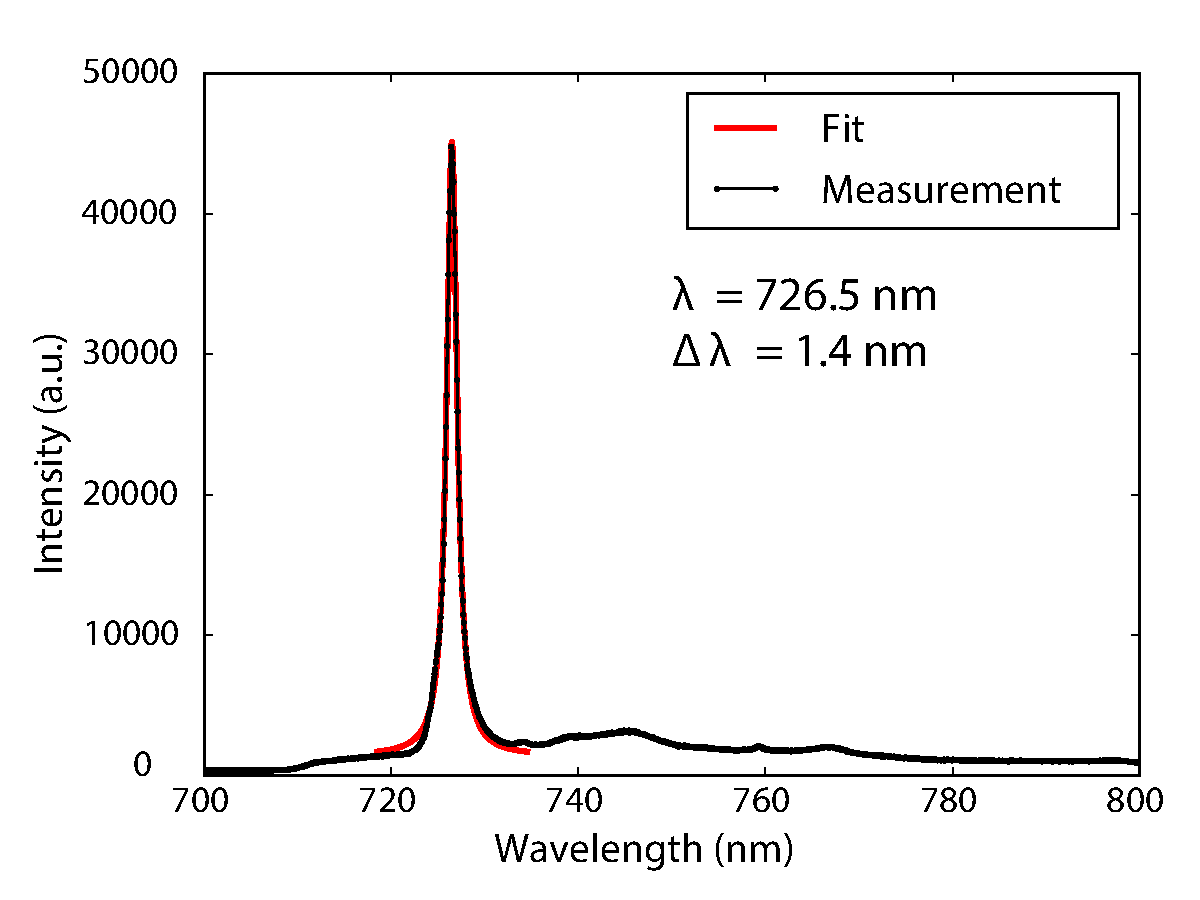
\includegraphics[trim = 0 0 0 0 , clip = true, width = \pairplotwide]{./pics/Ir8_Spektrum_8_notitle.pdf}}
			\caption{}\label{subfig::emnarrow}
		\end{subfigure}
		\hfill
		\begin{subfigure}{0.5\linewidth}
			\centering
			\testbox{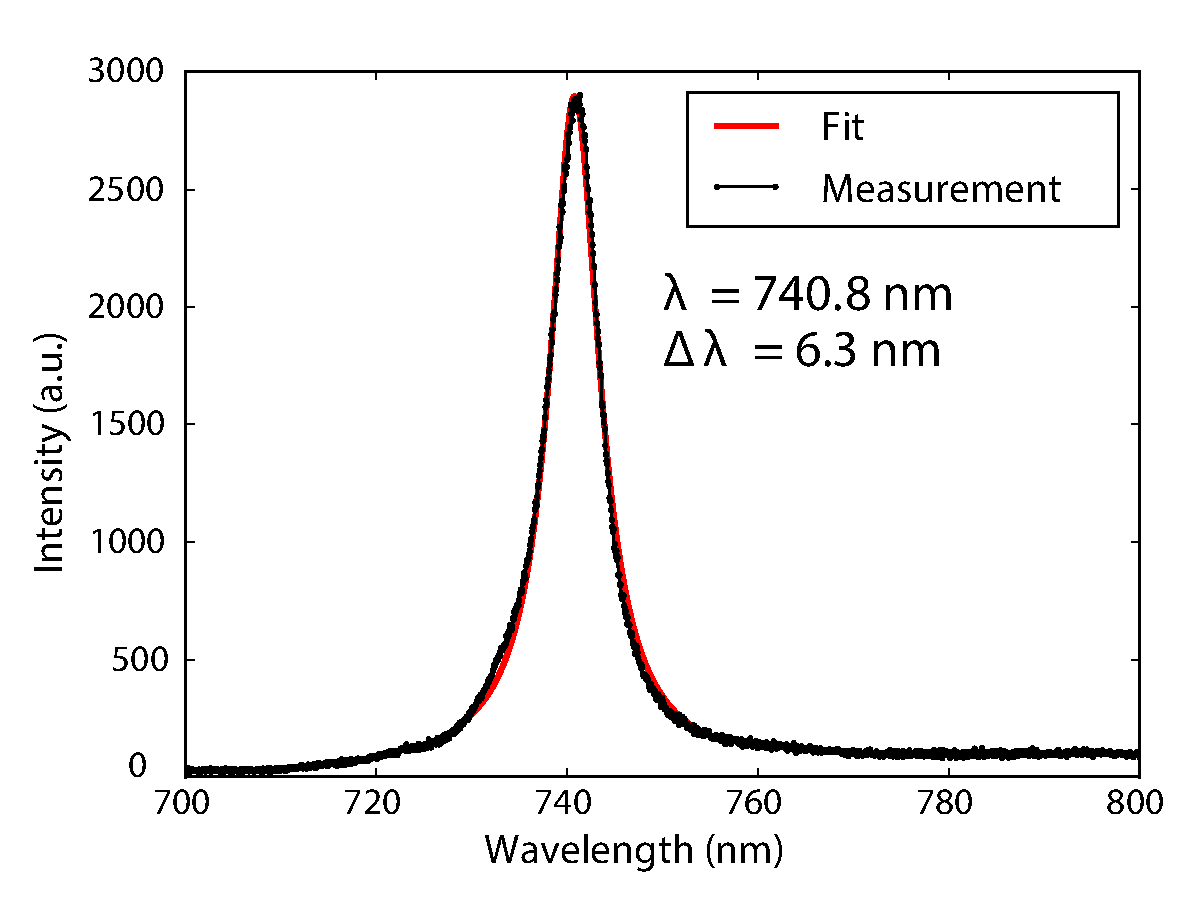
\includegraphics[trim = 0 0 0 0,  clip = true, width = \pairplotwide]{./pics/Ir8_scan_xy05_199uW_t30_notitle.pdf}}
			\caption{}\label{subfig::embroad}
		\end{subfigure}
		\caption[Sample \siv \pl spectra for \vl and \hl]{Representative photoluminescence spectra of sample \insituHao measured at room temperature. (a) Spectrum of \hl of \Fref{fig::bimodal_distr}, denoted \emnarrow. (b) Spectrum of \vl of \Fref{fig::bimodal_distr}, denoted \embroad. The red lines are Lorentzian fits to the peaks.}
		\label{fig::spectra}
	\end{figure}

	To determine how much the \ZPLs contribute to the total observed emission of \emnarrow and \embroad, we determine the \db factors for both.
	The \db factor is defined by $DW = I_{ZPL}/I_{TOT}$ and is therefore suited as a measure for sideband intensity.
	The \db factor for \emnarrow amounts to \num[separate-uncertainty]{0.81(1)} (given uncertainty due to fit).
	This \db factor corresponds to a \hr factor $S =- \ln{(DW)}$ \cite{Walker1979} of \num[separate-uncertainty]{0.21(1)}, which is in good agreement with the values reported in \cite{Neu2011b}.
	The error is mainly due to background corrections.
	When zooming in onto the spectrum of \embroad we do not find distinct sidebands peaks, i.e.\ almost all emission for this emitter is focused into the \ZPL.
	Considering resolution limits of the spectrometer, dark-counts and fluorescence background, we evaluate the \db factor to be larger than \num[separate-uncertainty]{0.97}.
	It is the largest \db factor amongst all our milled \sivs.
	The two mentioned \db factors should not be interpreted as single representative emitters for the respective groups, they rather serve as an orientation of the spread of the \db factors of both groups.
	It has to be pointed out, that we did not find any systematic difference of the \db factor between \hl and \vl.
	
	To provide context for the novel findings presented in \Fref{fig::bimodal_distr}, we compare our results to various earlier findings.
	Furthermore, we discuss an additional comparison to an investigated control sample fabricated using \si implantation.
	The results are presented in \Fref{fig::bimodal_distr_compare}.


	\begin{figure}[!htb]
		\centering
		\testbox{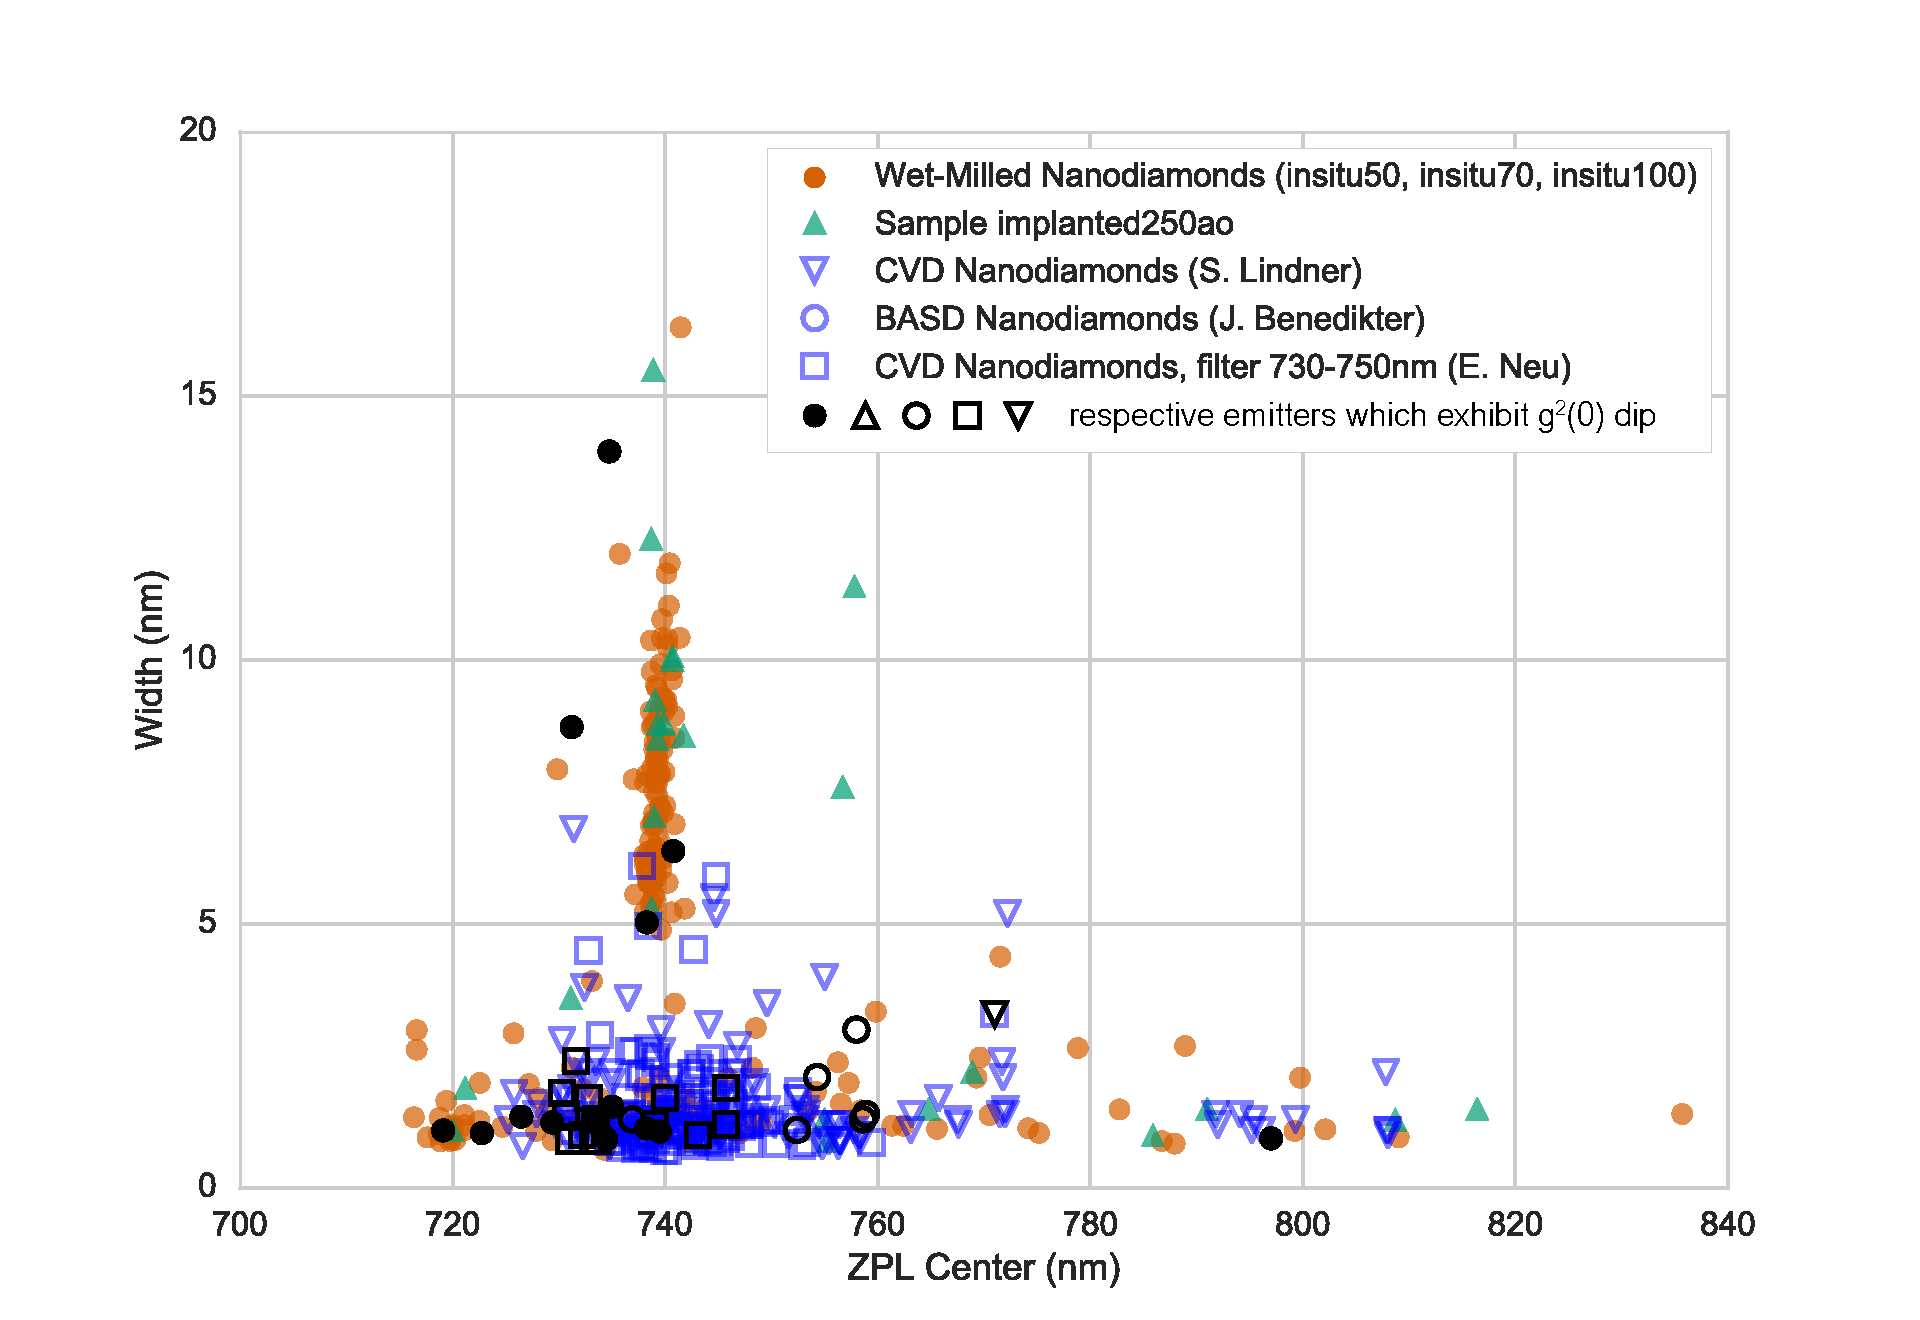
\includegraphics[trim = 0 0 0 0,  clip= true, width = \oneimagewide]{./pics/distro_alldata_three_colors_legend.pdf}}
		\caption[Comparison of \siv \lws with available data sources]{Comparison of the distribution of the \lw vs. the center wavelength of the ZPL of the investigated \sivs in milled \nds (samples \insituF, \insituS, \insituH) with data measured on sample \implantedTao (implanted with \Si); with data measured in our group on CVD \nds produced by M. Schreck \cite{Neu2011b}; with data measured on \nds reported by J. Benedikter in \cite{Benedikter2017a}; and with data measured in CVD diamonds by E. Neu in a filter window between \SIlist{730; 750}{nm} \cite{Neu2012}. Black symbols represent emitters exhibiting a dip in the \gtz function, indicating a single or very few \sivs}
		\label{fig::bimodal_distr_compare}
	\end{figure}


	Samples for which previous data has been taken are:
	\begin{enumerate}
		\item \nds produced by \basd (BASD) of polycrystalline \CVD diamond films (blue rings in \Fref{fig::bimodal_distr_compare} \cite{Neu2011a}; data taken from \cite{Benedikter2017a}).
		\item \label{item::elke_cvd}\nds produced by heteroepitaxial \CVD growth on \ir substrates with \textit{in-situ} incorporated \sivs; measured in a spectral filter window of \SIrange{730}{750}{nm} (blue squares in \Fref{fig::bimodal_distr_compare}; data reused from \cite{Neu2012} with permission).
		\item \nds produced in the same manner as in \ref{item::elke_cvd} (blue downwards pointing triangles in \Fref{fig::bimodal_distr_compare}; produced by M. Schreck \cite{Neu2011b}; spectroscopic measurement performed with setup described in \Fref{sec::confocal}).
	\end{enumerate}
	
	All previous data from different \nd material fit nicely with the \ZPL distribution presented in \Fref{fig::bimodal_distr_compare}, confirming the findings of \Fref{fig::bimodal_distr}.
	
		We verify that the observed luminescent defects are indeed \si related by performing control experiments with \si implanted samples (sample \implantedTao).
	By doing so we rule out the possibility that the two clusters in the distribution are a result of artifacts.
	Such artifacts include other elements incorporated into the \nds during the growth process: Residue from previous processes performed in the diamond growth chamber or material from chamber parts may be incorporated during \nd growth.
	\Fref{fig::bimodal_distr_compare} shows that the implanted \sivs cover roughly the same spectral range as the \textit{in-situ} incorporated centers from around \SIrange{720}{820}{nm} as the \textit{in-situ} incorporated centers.
	This correlation provides strong evidence for the \si related origin of the defects.
	
	% In the next paragraphs, the \ZPL distribution will be discussed in further detail.
	To provide a theoretical interpretation, the \ZPL \cwl shift is investigated in further detail and compared to results from density functional calculations.
	Zooming in to \vl (\Fref{subfig::distro_inset1}) it becomes clear that only six of the measured data points in \vl are situated at a shorter \cwl than the point attributed to an ideal \siv in unstrained bulk material.
	The the shortest wavelength shift is at \SI{729.9}{nm}.
	At the same time, much more data exhibit a \cwl bigger than the ideal \siv.
	This asymmetry suggests that a red-shift of the \ZPL of an \siv is significantly more likely than a blue-shift.

		\begin{figure}[!htb]
			\begin{subfigure}{.5\textwidth}
				\centering
				\testbox{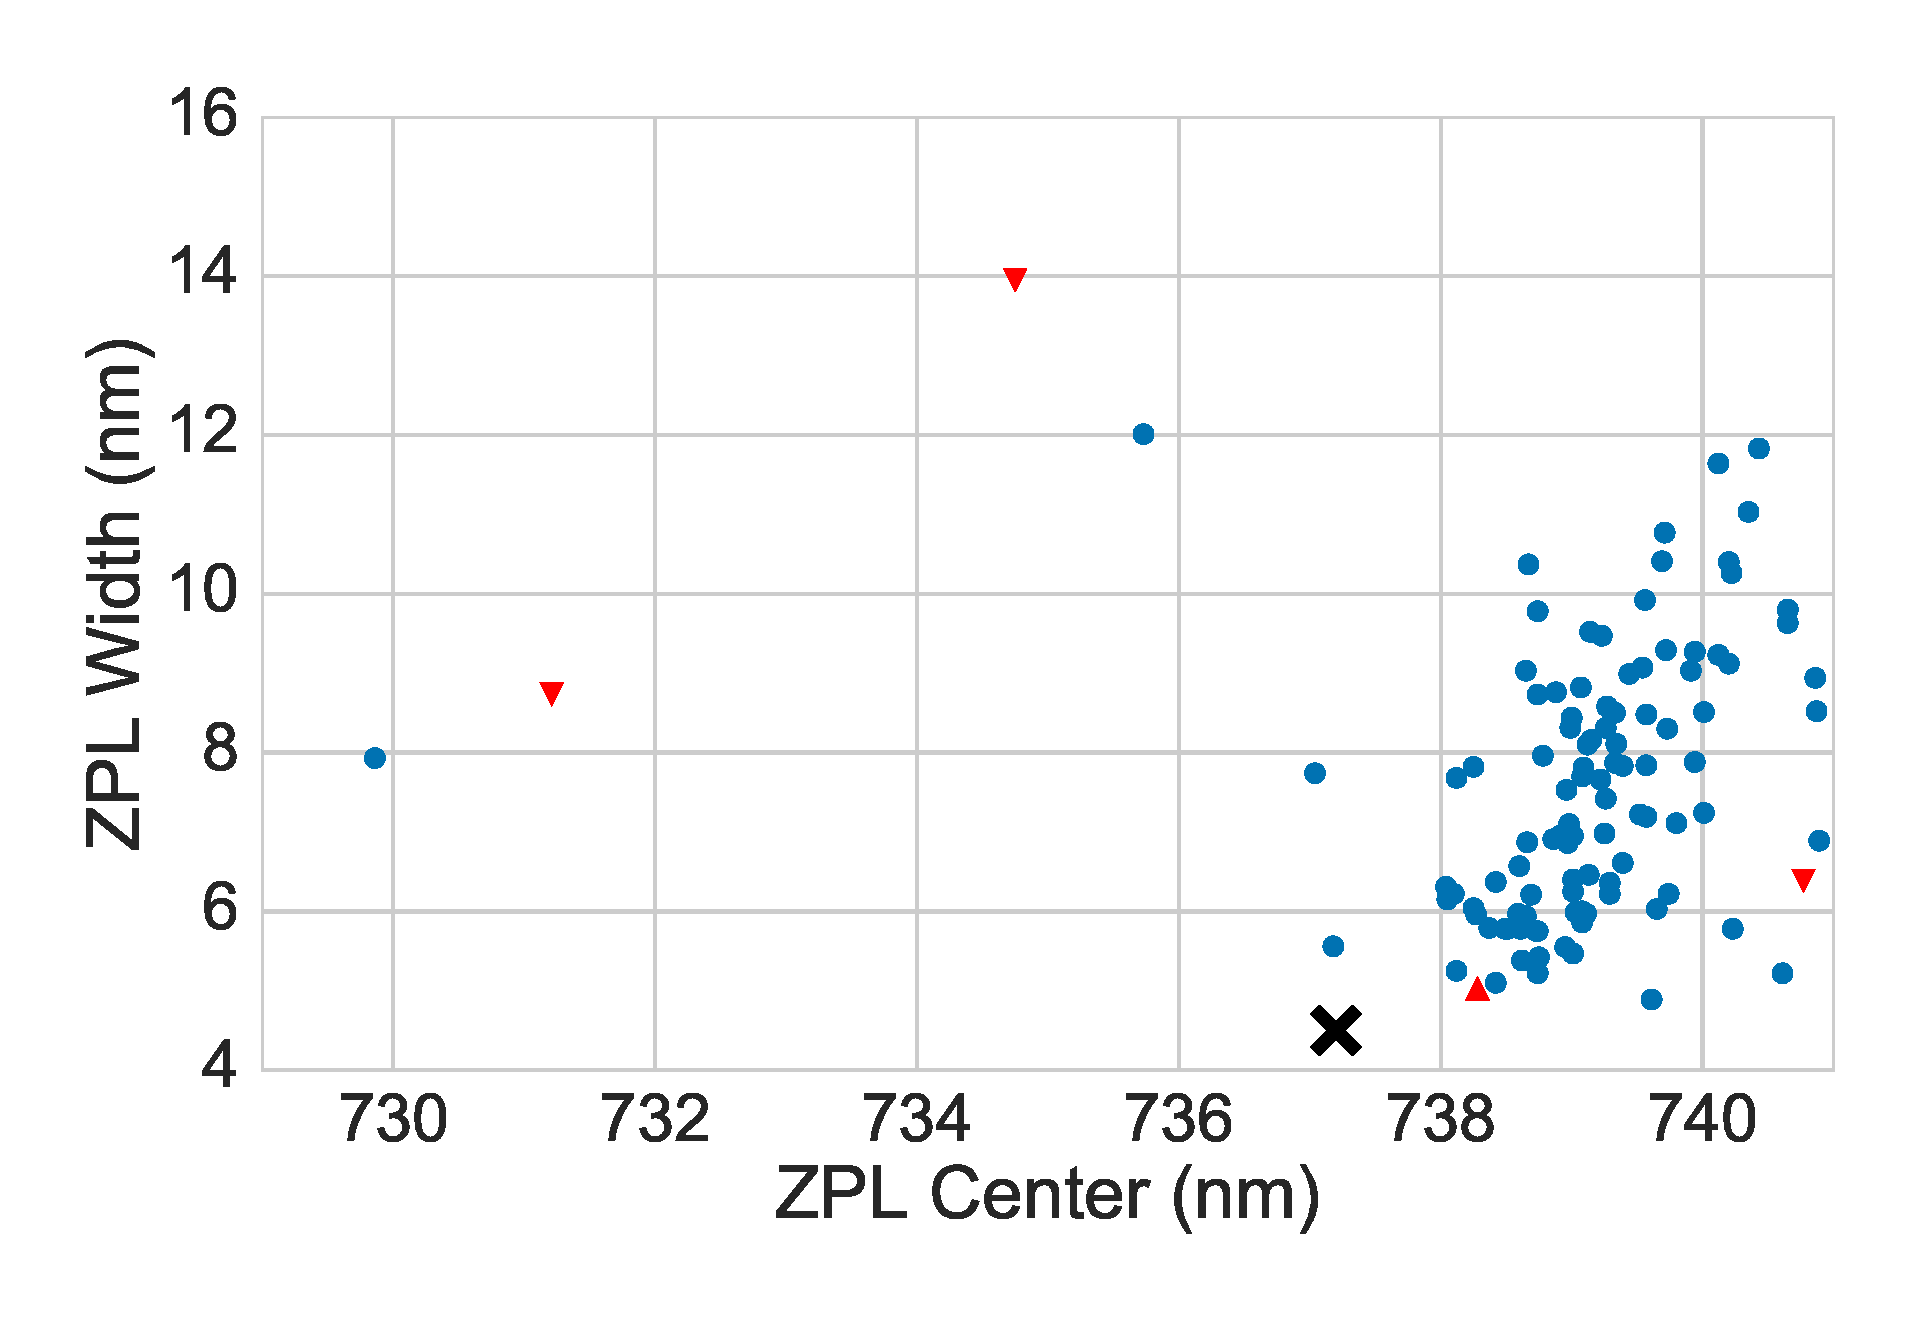
\includegraphics[trim = 0 0 0 0,  clip= true, width=\pairplotwide]{./pics/paper_inset_line_statistics_nofit.pdf}}
				\caption{}
				\label{subfig::distro_inset1}
			\end{subfigure}
			\begin{subfigure}{.5\textwidth}
				\centering
				\testbox{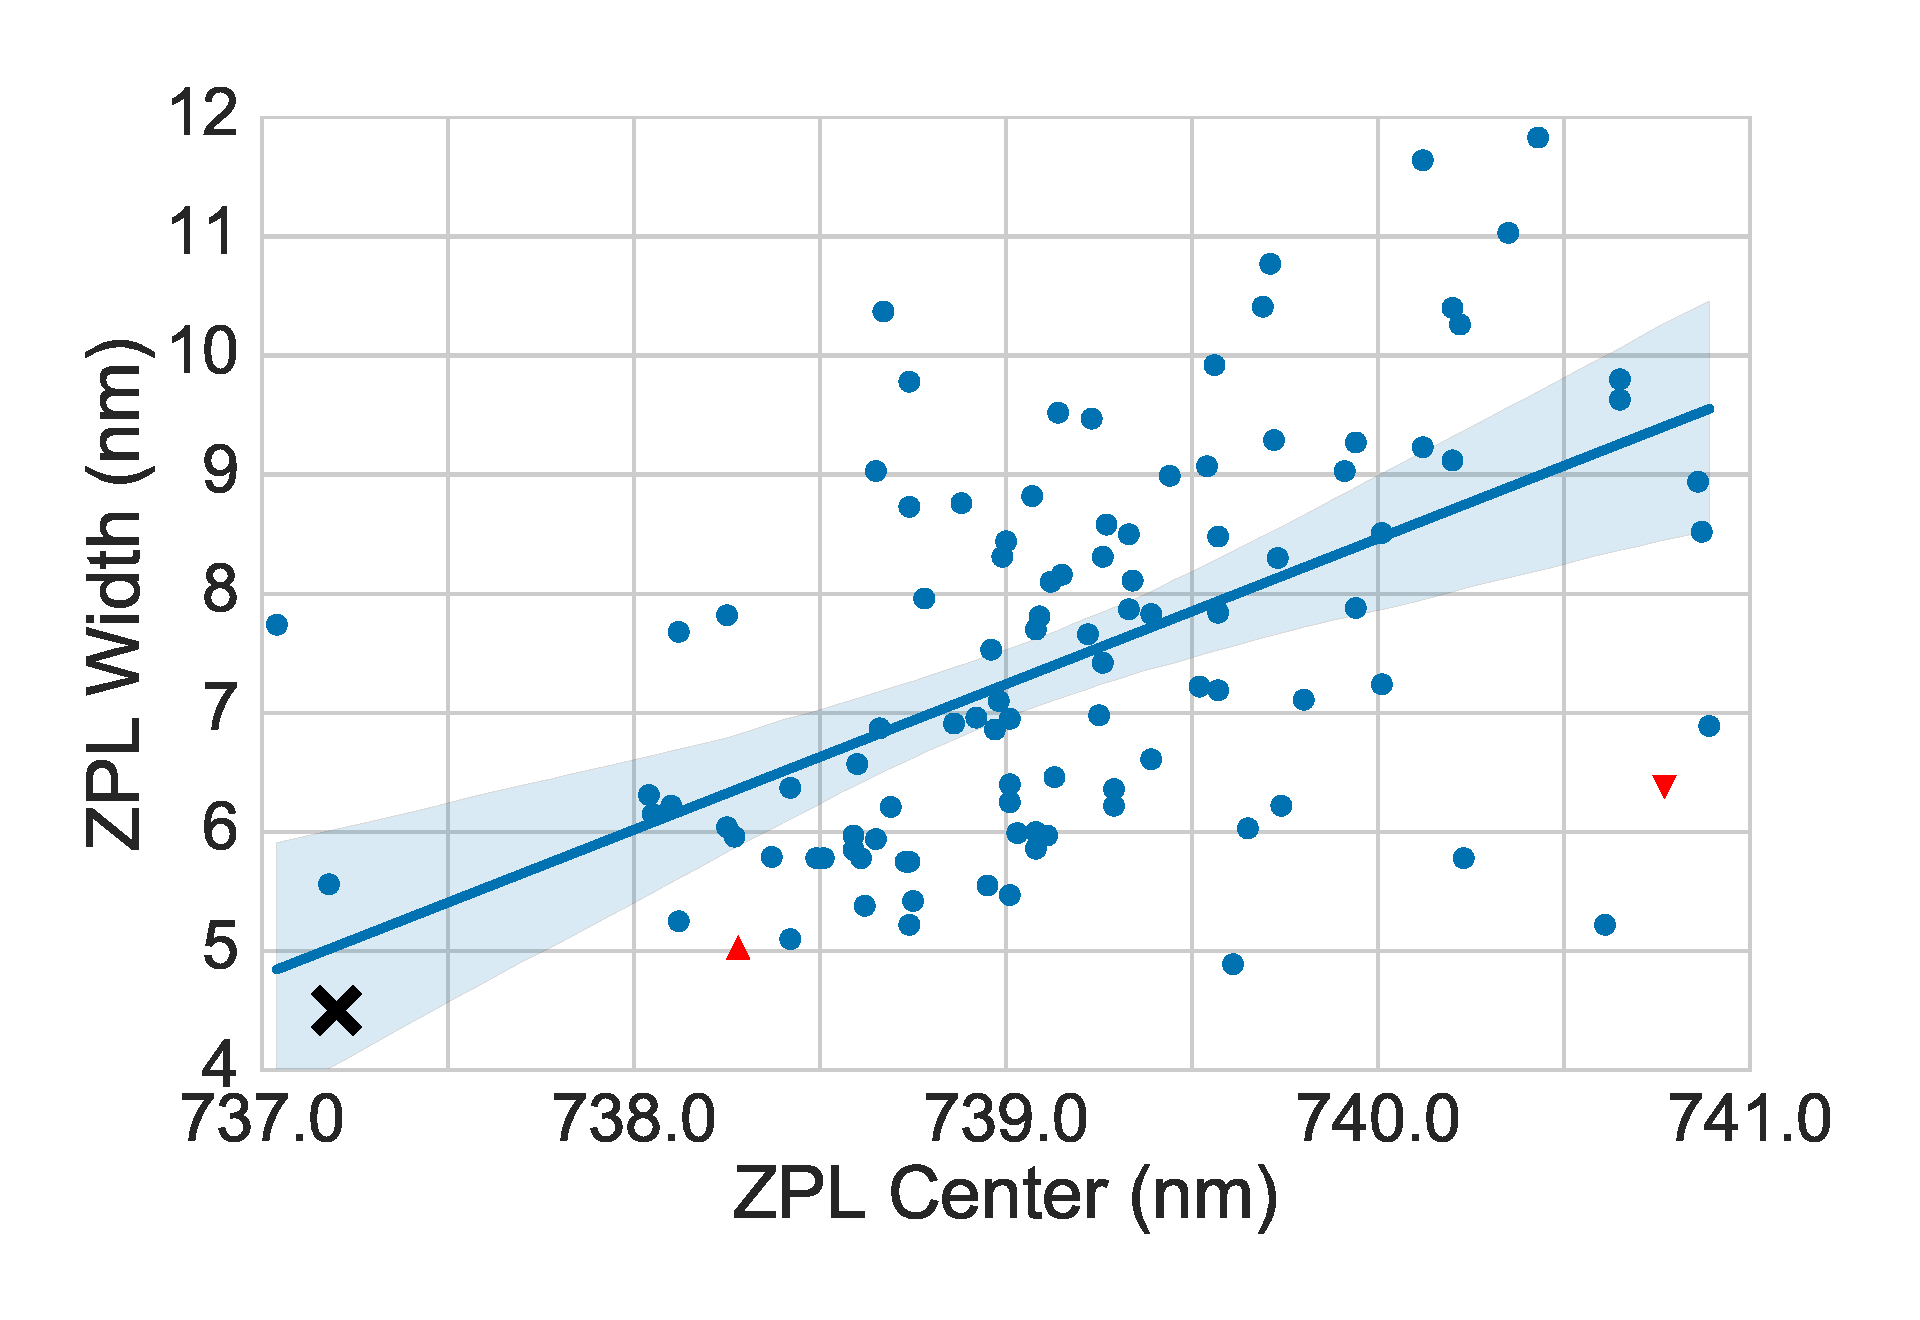
\includegraphics[trim = 0 0 0 0,  clip= true, width=\pairplotwide]{./pics/paper_line_statistics_regression.pdf}}
				\caption{}
				\label{subfig::distro_inset2}
			\end{subfigure}
			\caption[Zoom-in onto \sivs of the \vl]{(a) A zoom into \vl. While many data points exhibit higher \cwls (i.e. a redshift) than the ideal \siv in bulk, only few exhibit shorter \cwls (i.e. a blue-shift). (b) Zooming further into \vl, a clear trend of broader \ZPL \lws for larger \ZPL center shifts is visible. The line in a linear regression to all data points between \SIlist{737;741}{\nano\meter} which exhibit a \lw bigger than \SI{4}{\nano\meter}.}
			\label{fig::bimodal_distr_zoom}
		\end{figure}

	% Several mechanisms contribute to the \cwl shift, predominantly hydrostatic- and material strain.
	% As explained in \Fref{subsec::raman_strain}, we measured the Raman shift of samples \insituS and \implantedTao.
	% These measurements indicate strain in the diamond lattice in the range of \SIrange{-8.56}{4.26}{\giga\pascal}.
	% \Fref{fig::stress_pressure} shows results from density functional calculations.
	% The shift of the  \ZPL is modeled in dependence of pressure in the diamond lattice both for hydrostatic stress and for uniaxial stress.
	% \Fref{fig::stress_pressure} illustrates that the assumption stated in \Fref{subsec::raman_strain}, namely that the strain in the \nds is due to hydrostatic and uniaxial stress, corresponds well with the measured \ZPL shifts in \vl.

	% 	\begin{figure}[!htb]
	% 		\centering
	% 		\testbox{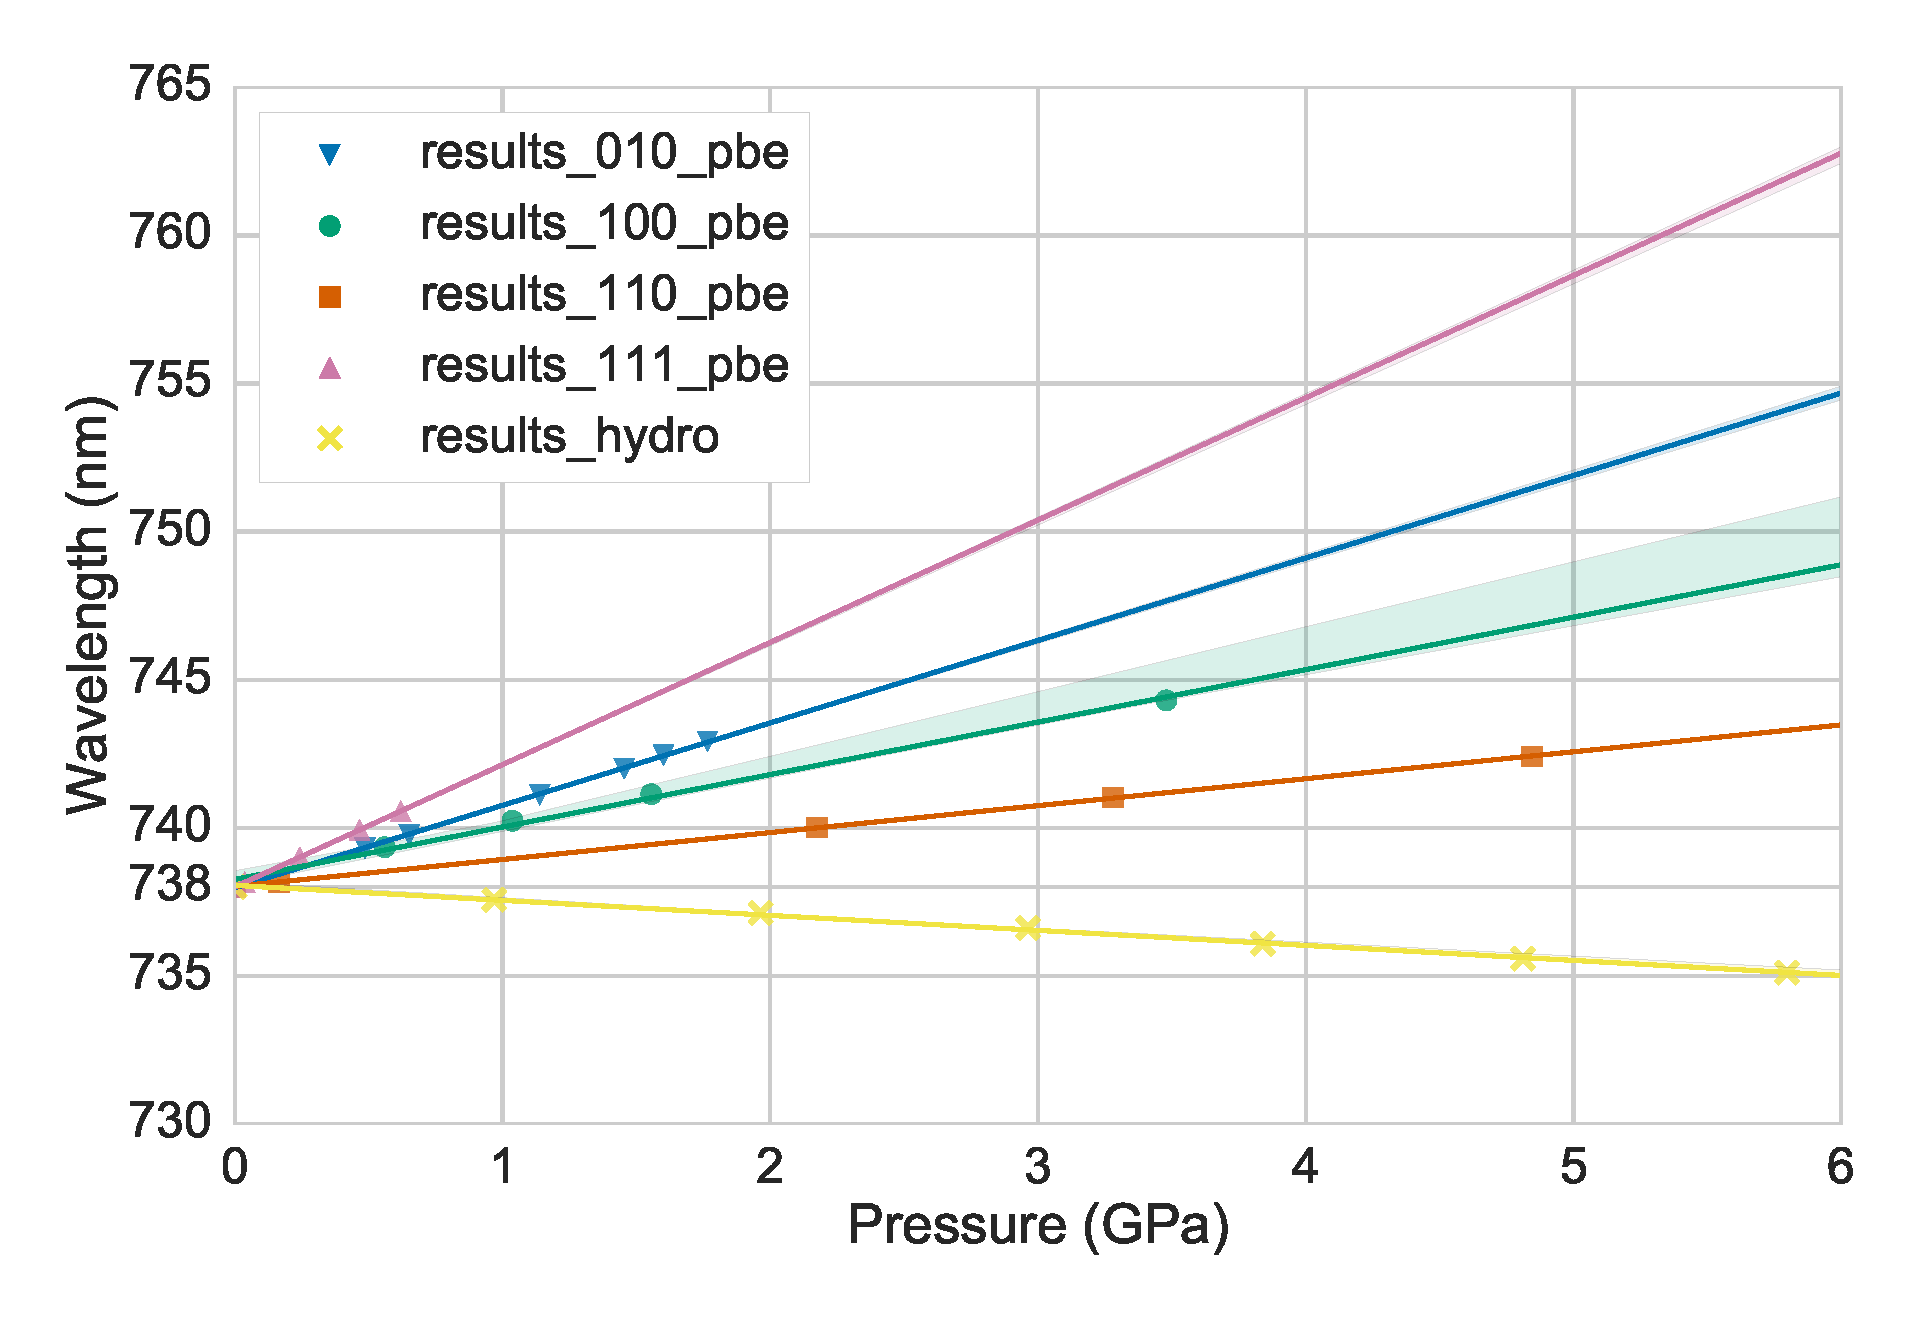
\includegraphics[trim = 0 0 0 0,  clip= true, width = 0.6\linewidth]{./pics/adam_gali_big_labels.pdf}}
	% 		\caption[Calculated dependence between \siv \ZPL and lattice pressure]{Calculations of the wavelength of the \siv \ZPL in dependence of pressure. Markers: calculated pressure with PBE functional; Lines: linear fits to the calculated points, the shaded area around the lines representing the one sigma (68\%) confidence interval. Yellow: hydrostatic pressure; other colors: uniaxial pressure, for different orientations. All calculations are performed with a PBE functional. Hydrostatic-type pressure causes a moderate blue shift whereas uniaxial strain causes larger redshift with different magnitudes depending on the direction of the strain}
	% 		\label{fig::stress_pressure}
	% 	\end{figure}

	% With higher uniaxial pressure, the \ZPL becomes more and more red-shifted.
	% The blue shifted \ZPL \cwls are explained by hydrostatic stress in the diamond material.
	% The strain calculated from the Raman measurements corresponds well with the results in \Fref{fig::stress_pressure} for \vl.
	% However, the measured shifts in \hl are too broad to be solely explained by strain in the diamond.
	% A potential explanation for the very broad distribution of defect center \ZPL \cwls could be the association of \sivs with a further nearby defect, such as a vacancy, or a modified SiV complex such as SiV:H \cite{Thiering2015}.
	% 
		% Zooming in to \vl, another effect becomes visible (\Fref{subfig::distro_inset2}):
	% With increasing  \ZPL \cwl, the \lw becomes broader.
	% As discussed above, a red-shift of the \ZPL is linked to increasing uniaxial strain.
	% Thus we conclude that the \ZPL \lw too is affected by strain in the diamond lattice.
	% Here, a modified electron-phonon coupling \cite{Jahnke2015a} causes increased uniaxial stress, resulting in larger \lws.
	% A similar effect has been previously observed for \sivs at cryogenic temperatures \cite{Arend2016a}.
	% 
		% To conclude, we are able to explain the distribution of \ZPL \cwls in \vl very consistently with theoretical predictions based on perturbative shifts due to strain in the diamond lattice.
	% On the other hand, we have to assume that \hl is comprised of modified \sivs, the structure of which is currently unclear.
	
	
	Several mechanisms contribute to the \cwl shift, predominantly hydrostatic- and material strain.
	As discussed in \Fref{subsec::raman_strain}, we measured the Raman shift of samples \insituS and \implantedTao.
	These measurements indicate strain in the diamond lattice in the range of \SIrange{-8.33}{5.27}{\giga\pascal}.
	In the following, we first discuss the stress/strain shift mechanisms for the \siv before we compare theoretically derived strain shift coefficients to the mentioned range of \ZPL shifts.

	To gain insight into the strain mechanism for \sivs in diamond, we perform ab initio Kohn-Sham density functional theory (DFT) calculations on the strain \ZPL shift coupling parameters. 
	The unstrained model of the negatively charged \sivc (SiV$^{-}$) in bulk diamond is constructed starting from a $512$ atom pristine diamond simple cubic supercell within the $\Gamma$ point approximation. 
	The $\Gamma$ point sampling of the Brillouin zone has proven to be adequate for defects in $512$-atom supercells \cite{deak2014formation,kaviani2014proper} providing a sufficiently converged charge density. 
	The SiV$^{-}$ defect has $S=1$ and it is found to have $D_{3d}$ symmetry with an axis oriented along  $\langle 111 \rangle$ \cite{Goss2007}. 
	Standard projector augmented-wave (PAW) formalism together with plane waves are applied, as implemented in the Vienna Ab initio Simulation Package (VASP) code \cite{kresse1993ab,kresse1996efficiency,kresse1996efficient,kresse1999ultrasoft}. The geometry optimization is carried out within the constructed supercell by using the Perdew-Burke-Ernzerhof (PBE) DFT functional \cite{perdew1996generalized}. A \SI{420}{\eV} cutoff is applied for the wave function expansion and a \SI{1260}{\eV} cutoff for the charge density. The geometry of the defect is optimized until the forces were lower than \SI{d-6}{\eV\per\angstrom}. The $D_{3d}$ symmetry is preserved for both the ground state and the excited state after relaxation.

	The ground state of the defect is found to have electronic configuration $e^{4}_{u} e^{3}_{g}$ (${}^{2}E_{g}$) while the excited state is modeled by promoting one electron from the $e_u$ to the $e_g$ level and presents electronic configuration  $e^{3}_{u} e^{4}_{g}$ (${}^{2}E_{u}$). Both these states are dynamic Jahn-Teller systems \cite{Hepp2014, Rogers2014a}. The optical signal of the defect (\ZPL) can be calculated as the lowest excitation energy by the constraint DFT approach (CDFT) \cite{gali2009theory}. According to CDFT one electron is promoted from the ground state to a higher level leaving a hole behind. The interaction between the electron and the hole is included in the procedure. The \ZPL energies were obtained by taking the total energies of the optimized geometries in the ground and excited state.

	The strain on the defect structure is simulated by applying a compression to the supercell along a well defined direction. The strained supercells are obtained by compressions along $\langle 100 \rangle$, $\langle 110 \rangle$ and $\langle 111 \rangle$. We also study the configuration produced by a hydrostatic pressure, which consists in subjecting the cell to the same compression along the three directions. After introducing the strain along the directions, the ZPL energies were calculated for each strained supercell. Finally, we obtained data points on the calculated \ZPL energies vs. the applied strain. These \ZPL energies correspond to the optical transition between the lower branch levels of the ${}^{2}E_{u}$ and ${}^{2}E_{g}$ doublets. We note that additional calculations were performed for the  $\langle 100 \rangle$ and  $\langle 110 \rangle$ strained supercells by using the screened, range-separated, non-local hybrid density functional of Heyd-Scuseria-Ernzerhof (HSE06) \cite{heyd2003hybrid,krukau2006influence} and we found good agreement with the PBE values.

	Nudged elastic band (NEB) calculations \cite{henkelman2000climbing} by HSE06 were performed in order to calculate the energy barriers in the ground state in strained supercells. The barrier energies between the $C_{2h}$ configurations stayed under \SI{10.0}{\meV} which implies small change in the adiabatic potential energy surface around the $D_{3d}$ symmetry upon the applied strain. As a consequence, the Ham reduction factor in strained \siv will minutely change with respect to that of unstrained \siv \cite{thiering2018ab}. This suggests that the observed \ZPL shifts upon stress are directly strain related, and the contribution of the change of the effective spin-orbit to the \ZPL shifts is minor.

	\begin{figure}[!htb]
		\centering
		\testbox{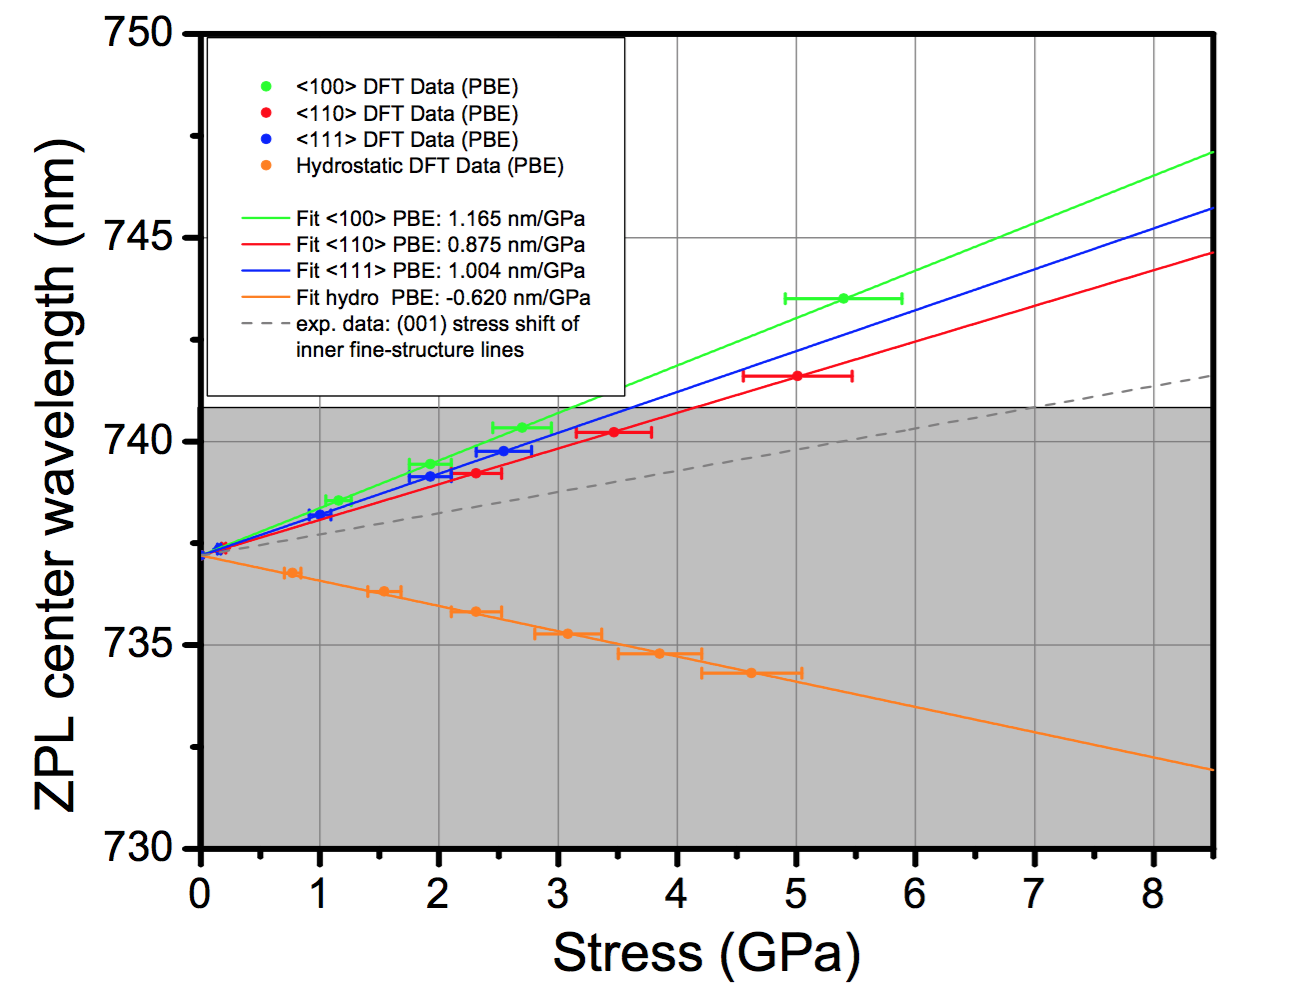
\includegraphics[trim = 0 0 0 0,  clip= true, width = \linewidth]{./pics/gali_calculations_new.png}}
		\caption[Calculated dependence between \siv \ZPL and lattice pressure]{Calculations of the \wl of the \siv \ZPL in dependence of pressure. Markers: DFT calculated pressure with PBE and HSE functionals; Lines: linear fits to the calculated points. Hydrostatic-type pressure causes a moderate blue shift whereas uniaxial strain causes larger redshift with different magnitudes depending on the direction of the strain. Grey line: experimental stress shift data for $\langle 001 \rangle$ uniaxial stress and inner fine-structure line of the \siv. Grey area: range of \ZPL center wavelengths of \vl.}
		\label{fig::stress_pressure}
	\end{figure}

	The data points in \Fref{fig::stress_pressure} show \ZPL \cwl shifts calculated with the method outlined above. For comparison with experimentally determined stress data the strain values of the theoretical calculation were converted into stress assuming a simplified model where diamond is approximated as isotropic linear elastic material. In this case stress $\sigma$ is related to strain $\epsilon$ via Young’s modulus as
% 
	\begin{equation}
		\sigma = E \epsilon .
	\end{equation}

	This assumption is pragmatic as we do not know the orientation of stress in the \nds from the Raman measurements but only its modulus. The values of $E$ vary considerably among different diamond materials \cite{hess2012mechanical} but even nanocrystalline diamond may obtain a large Young’s modulus $E \geq \SI{1000}{\GPa}$ \cite{williams2010high}. As an average value for the \nd size used in our investigations we assume $E = \SI[separate-uncertainty]{1000+-100}{\GPa}$ \cite{hess2012mechanical}. The calculated data points were extrapolated by linear fit functions to yield stress shift coefficients for the range of stress (up to $\approx \SI{8.5}{\GPa})$ found in the \nds. The grey area covers the \wl range of experimental \ZPL \wls measured within \vl. The dashed grey line represents stress-shifts of \siv emission lines at low temperatures derived from the only experimentally measured stress shift coefficient for the \siv under uniaxial stress in $\langle 001 \rangle$ \cite{Sternschulte1994,Hepp2014}. 
	The measurements of \cite{Sternschulte1994} were performed at \SI{4}{\kelvin} and reveal the shifts of the \siv fine structure lines: the outer lines of this fine structure shift with about \SI{4}{\nm\per\GPa} (\SI{2.23}{\THz\per\GPa}, not shown here), whereas the inner lines shift with only \SI{0.52}{\nm\per\GPa} (\SI{292}{\GHz\per\GPa}, denoted as dashed line). The room temperature spectrum, however, is mostly governed by the inner line ``C'' of the spectrum \cite{Arend2016a}, i.e.\ the line with second highest \wl, corresponding to the optical transition between the lower branch levels of the ${}^{2}E_{u}$ and ${}^{2}E_{g}$ doublets as used in the DFT calculations. We find that the calculated uniaxial stress shift coefficients match well the experimentally obtained value (dashed line) and both coincide well with the range of measured red-shifted \ZPLs of \vl (grey area). We thus interpret the \ZPL shifts of \vl as originating from level shifts due to uniaxial strain. 
	Furthermore, the calculated \ZPL shifts due to hydrostatic pressure coincide well with the range of the blue shifted \ZPLs that we observe in \vl. The fact that we see only few blue-shifted \ZPLs might be due to reason that pure hydrostatic pressure is rarely observed and overlayed by uniaxial stress in the \nds. 
	On the other hand, the measured shifts in \hl are too broad to be solely explained by strain in the diamond. A potential explanation for the very inhomogeneous distribution of defect center \ZPL \cwls could be the association of \sivs with a further nearby defect, such as a vacancy, or a modified SiV complex such as SiV:H \cite{Thiering2015}.

	Zooming in to \vl, another effect becomes visible (\Fref{subfig::distro_inset2}):
	With increasing  \ZPL \cwl, the \lw becomes broader.
	As discussed above, a red-shift of the \ZPL is linked to increasing uniaxial strain.
	Thus we conclude that the \ZPL \lw too is affected by strain in the diamond lattice.
	Here, a modified electron-phonon coupling \cite{Jahnke2015a} causes increased uniaxial stress, resulting in larger \lws.
	A similar effect has been previously observed for \sivs at cryogenic temperatures \cite{Arend2016a}.
	
	To conclude, we are able to explain the distribution of \ZPL \cwls in \vl very consistently with theoretical predictions based on perturbative shifts due to strain in the diamond lattice.
	On the other hand, we have to assume that \hl is comprised of modified \sivs, the structure of which is currently unclear.
